\documentclass{article}
\usepackage[utf8]{inputenc}

\title{wander}
\author{Thomas Eskridge}
\date{November 2018}

\usepackage{natbib}
\usepackage{graphicx}

\begin{document}

\maketitle

\section{Introduction}

main idea is an IDE for ontology viewing and class construction
Properties of IDE
\begin{enumerate}
    \item Structure source according to views
    \begin{itemize}
        \item Lexical: 
        \item Call graph
        \item modules
        \item file
        \item method
    \end{itemize}
    \item navigate between named components
\end{enumerate}

\begin{figure}[h!]
\centering
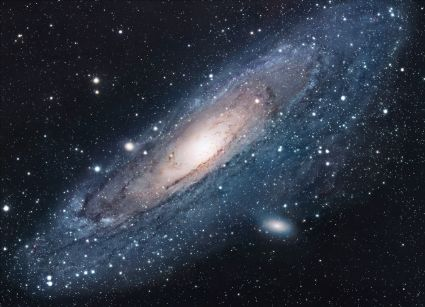
\includegraphics[scale=1.7]{universe}
\caption{The Universe}
\label{fig:universe}
\end{figure}

\section{Conclusion}
``I always thought something was fundamentally wrong with the universe'' \citep{adams1995hitchhiker}

\bibliographystyle{plain}
\bibliography{references}
\end{document}
